%% Full length research paper template
%% Created by Simon Hengchen and Nilo Pedrazzini for the Journal of Open Humanities Data (https://openhumanitiesdata.metajnl.com)

\documentclass{article}
\usepackage[english]{babel}
\usepackage[utf8]{inputenc}
\usepackage{johd}
\usepackage{float}
\usepackage{adjustbox}
\usepackage{amsmath}

\title{Determining the number of roots of a given polynomial through its newton fractal and deep-learning techniques}

\author{Roque Mula, Marco Nieto, Pablo Pérez \\
        \small Physics engeneering degree, Polythecnic University of Valencia. \\
}

\date{} %leave blank

\begin{document}

\maketitle

\begin{abstract} 
\noindent A short (up to 250 words) summary of the main contributions of the paper and the context of the research. Full length papers discuss and illustrate methods, challenges, and limitations in the creation, collection, management, access, processing, or analysis of data in humanities research, including standards and formats. These aspects must not necessarily be discussed with reference to a specific dataset (or collection thereof) but, if your paper focusses on particular datasets, we advise to add the dataset metadata under the section ‘Dataset description’. This template provides a general outline for full length papers and authors can adapt the headings and include subheadings as they find appropriate. Please delete or replace the blue text with your own text in black.  \end{abstract}

\noindent\keywords{newton fractal; machine learning; neural network}\\


\section{Context and motivation}

The main motivation of this paper is the curiosity on the fractal behaviour that emerges from a extremely simple function such as a polynomial. The brand new techniques and practical uses that are being developed in deep learning and AI suits perfectly this context, as image recognizing is a well-studied topic in this field.

\subsection{About the Newton's Fractal}

\noindent The Newton fractal\footnote{which Newton did not see in life despite having his name} is a classification of the points that comprise the complex plane, characterized by the application of Newton's method to fixed polynomials \hyperref[id1]{[1]}. When there are no attractive cycles, it divides the complex plane into  $\{n_0, n_1, ..., n_i, ... n_{-k}, n_k\}$ regions , each of which is associated with a root $i$ of the polynomial of order $k$. In this way, Newtonian fractals resemble Mandelbrot sets and, like other fractals, exhibit complex appearances derived from simple descriptions. It is relevant to numerical analysis because it shows that outside the region of quadratic convergence \hyperref[id2]{[2]}, Newton's method is very sensitive to the starting point choice.

\vspace{10}
\noindent The Newton-Raphson method is performed in this way: An initial point is arbitrarily chosen, and this point is used as the initial value $z_0$ for Newton iterations 
\begin{center}
\begin{equation*}
\scalebox{1}{$Z_{n+1}=Z_n-\frac{p(z)}{p'(z)}$} 
\end{equation*}
\end{center}
\vspace{10}
giving a sequence of points $\{z_1 , z_2 , ...\}$ if the sequence converges to the root $i$ , then $z_0$ is an element of the region $n_i$. However, for every polynomial of degree at least 2 there are points for which the Newton iteration does not converge to any root. This method is widely used to compute the roots of polynomial functions ob arbitrary orders, not only in one dimension but higher. Some of its applications are estimating linear regression models, optimization problems or adjusting the parameters of many simulations or machines. \hyperref[id3]{[3]}
\vspace{10}

\noindent The fractal behaviour emerges with polynomials of order equal or higher than 3. This is caused because the boundaries of every region $n_i$ are always adjacent to each other root regions, and the only way to preserve this propierty, independently of the scale, is the image to have infinite complexity on its boundaries.
That's why with polynomials of order 2 the complex patterns do not appear, because the boundary between the two regions is a straight line, as it's the simplest way to have the two regions in contact.


\begin{figure}[h!]
\centering
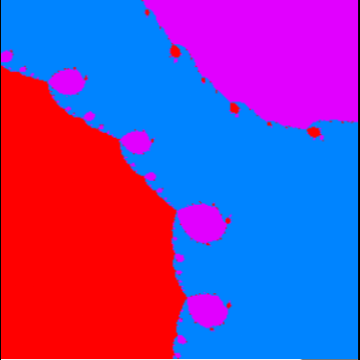
\includegraphics[width=5cm,height=5cm]{images/g3_1.jpg}
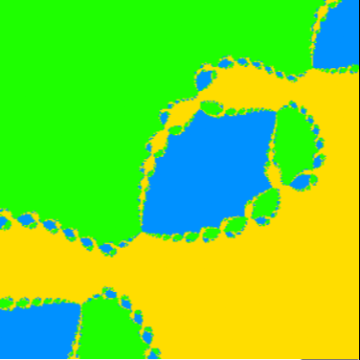
\includegraphics[width=5cm,height=5cm]{images/g3_2.jpg}
\caption{Examples of Newton Fractals, computed from the functions $\frac{(x^2-1)(x^2+1)}{2x((x^2-1)+(x^2+1))}$} (left) and $\frac{x^3-1}{3x^2}$ (right), between the limits 2,-2, $2i$, $-2i$.
\label{exnewton}
\end{figure}


\section{Technical tools and resources}
For this work, a recently created software has been fundamental in some parts. The chatbot 'ChatGPT' developed by the company OpenAI has been used to generate some parts of the code, to give a general overview of the topics that we had to deepen on and to generate some examples in order to make our contributions as similar as possible to already stablished standards in the field. More information about this tool can be found at \href{https://openai.com/blog/chatgpt/}{OpenAI's chatGPT main page}.

\noindent For the data generation, the javascript program 'Interactive Newton Fractal'\hyperref[id4]{[4]},developed by the user 'SingularPTS' has been used. It consists in an interactive app that lets the user choose the desired number of roots and colour them in any colour palette
For the deep-learning and implementation of neural networks, the python library 'TensorFlow', and more specifically the 'Keras' model has been used.

\noindent All the files containing the code needed for this article can be found inside the \texttt{GitHub} repository \href{https://github.com/Mnietoprez/newton-fractal-deep-learning}{newton-fractal-deep-learning}.

\section{Dataset description}
\subsection{Image processing}
As the interactive fractal builder used to generate the images did not have an option to directly save the generated plot, images have been stored using manual screenshots and a posterior resizing. An online image resizer has been necessary in order to preserve the same ratio among the images, 360x360 pixels.

\vspace{10}
\noindent It is well known that training an artificial intelligence has an add-on of difficulty because of the extreme care that has to be put in the quality of training data sources. For our results to be more precise, we have considered that providing the model colored images would not be the best option, because we don't want the model to learn how to distinguish between colors, but figures and patterns that emerge with Newton fractals. That's why all the data provided to the model has been processed with a Sobel filter, which converts the original image to a black and white picture where the edges of the shapes are remarked.

\begin{figure}[h!]
\centering
\includegraphics[width=4.5cm,height=4.5cm]{images/nosobel.png}
\hspace{6}
\includegraphics[width=4.5cm,height=4.5cm]{images/sobel.png}
\centering
\caption{Example of a Sobel filter applyed to a Newton fractal.}
\label{exnewton}
\end{figure}

\noindent The sobel filter technique consists in convolving the original image with two 3x3 matrix kernels:

\begin{center}
\begin{equation*}
$\textbf{G}_x =$ \begin{bmatrix}
+1 & 0 & -1\\
+2 & 0 & -2\\
+1 & 0 & -1\\
\end{bmatrix} 
\hspace{10}
$\textbf{G}_y =$ \begin{bmatrix}
+1 & +2 & +1\\
0 & 0 & 0\\
-1 & -2 & -1\\
\end{bmatrix} 
\end{equation*}
\end{center}
$\textbf{G}_x$ is used to calculate derivative approximations in the horizontal changes, and $\textbf{G}_y$ in the vertical changes. This computations have been performed automatically using functions from the 'cv2' and 'numpy' python libraries.



\subsection{Data organization}

\section{Neural network description}
Describe the methods used in the study.

\section{Results and possible applications}
Describe and discuss the results of the study.


\bibliographystyle{johd}
\bibliography{bib}
\vspace{10}

\noindent\label{id1}[1] Interactive Newton Fractal, developed by 'SingularPTS'. \href{https://editor.p5js.org/SingularPts/sketches/3wWBB8YRP}{https://p5js.org/es/}
\vspace{10}

\noindent\label{id2}[2] Roland Hildebrand: Local convergence behaviour of the Newton method. \href{http://ru.discrete-mathematics.org/nir/hildebrand.pdf}{https://mipt.ru/}
\vspace{10}

\noindent\label{id3}[3] Michael McAleer: Applications of the Newton-Raphson Method in Decision Sciences and Education. \href{https://iads.site/wp-content/uploads/papers/2019/Applications-of-the-Newton-Raphson-Method-in-Decision-Sciences-and-Education.pdf}{https://iads.site/}
\vspace{}

\noindent\label{id4}[4] J. Hubbard, D. Schleicher, S. Sutherland: How to find all roots of complex polynomials by Newton’s method. \href{https://www.semanticscholar.org/paper/How-to-find-all-roots-of-complex-polynomials-by-Hubbard-Schleicher/227bd87bed09b7541725ac3bd30dc145f9a984d7}{https://www.semanticscholar.org/}
\vspace{10}


\end{document}